\documentclass{article}
\usepackage{graphicx} % Include the graphicx package
\usepackage{float} % Include the float package for H option
\usepackage{subfiles} % Include the subfiles package for subfile management

% Set the graphics path to the current directory
\graphicspath{{./}}
\begin{document}

\title{Operational NMOS amplifier with NMOS differential pair}
\maketitle

\section{current bias generation characteristic's}

Fig.\ref{fig:values} represents the minimum voltage allowed for the current reference to work as supposed.

\begin{figure}[H] % Use H option for float placement
    \centering
    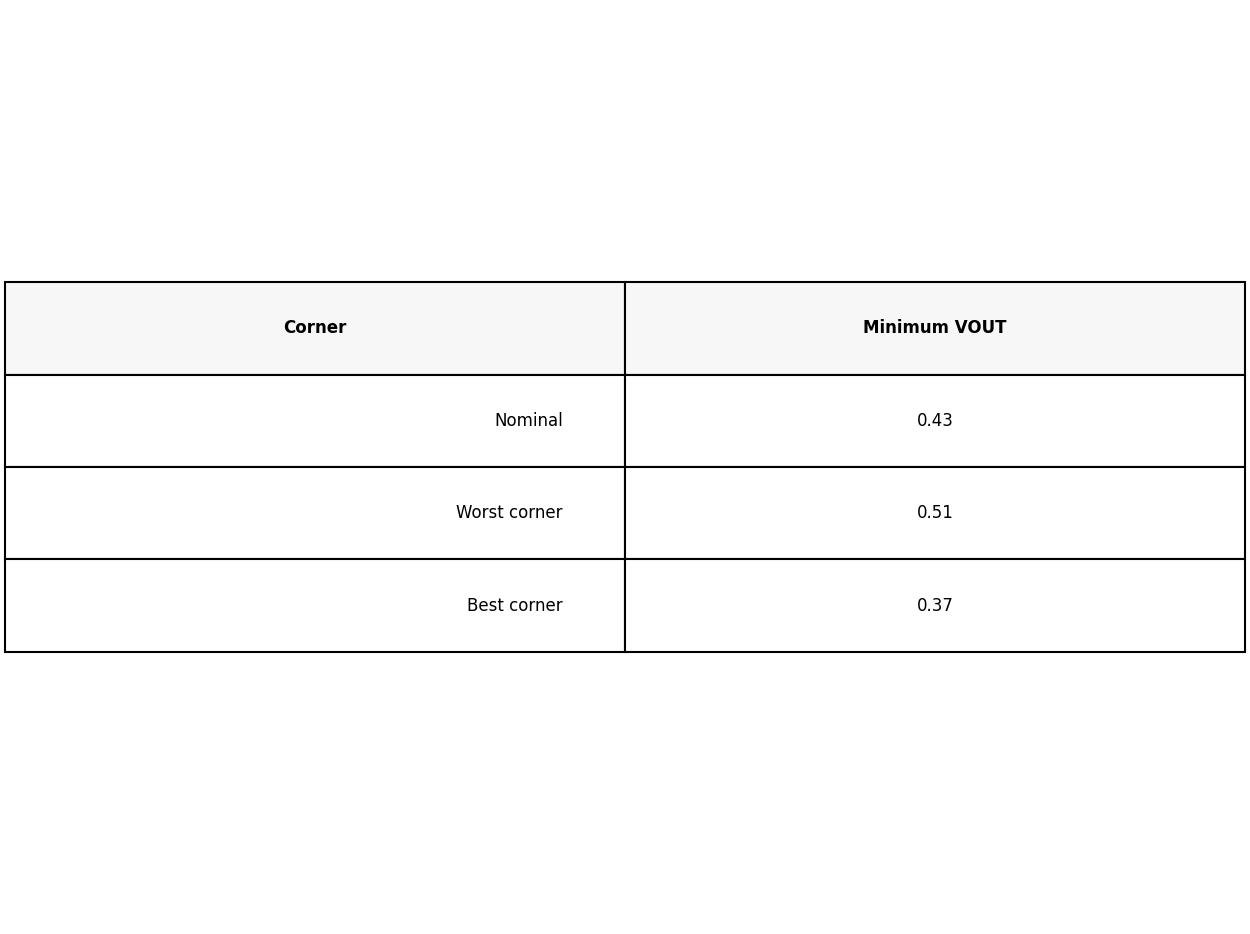
\includegraphics[width=.7\textwidth]{./interception_table.jpg} % Assuming this is the image generated by your Python script
    \caption{minimum voltage}
    \label{fig:values}
\end{figure}




Fig.\ref{fig:iout_vs_vout} represent the output current characteristic fo nominal, worst and best case scenario.

\begin{figure}[H] % Use H option for float placement
    \centering
    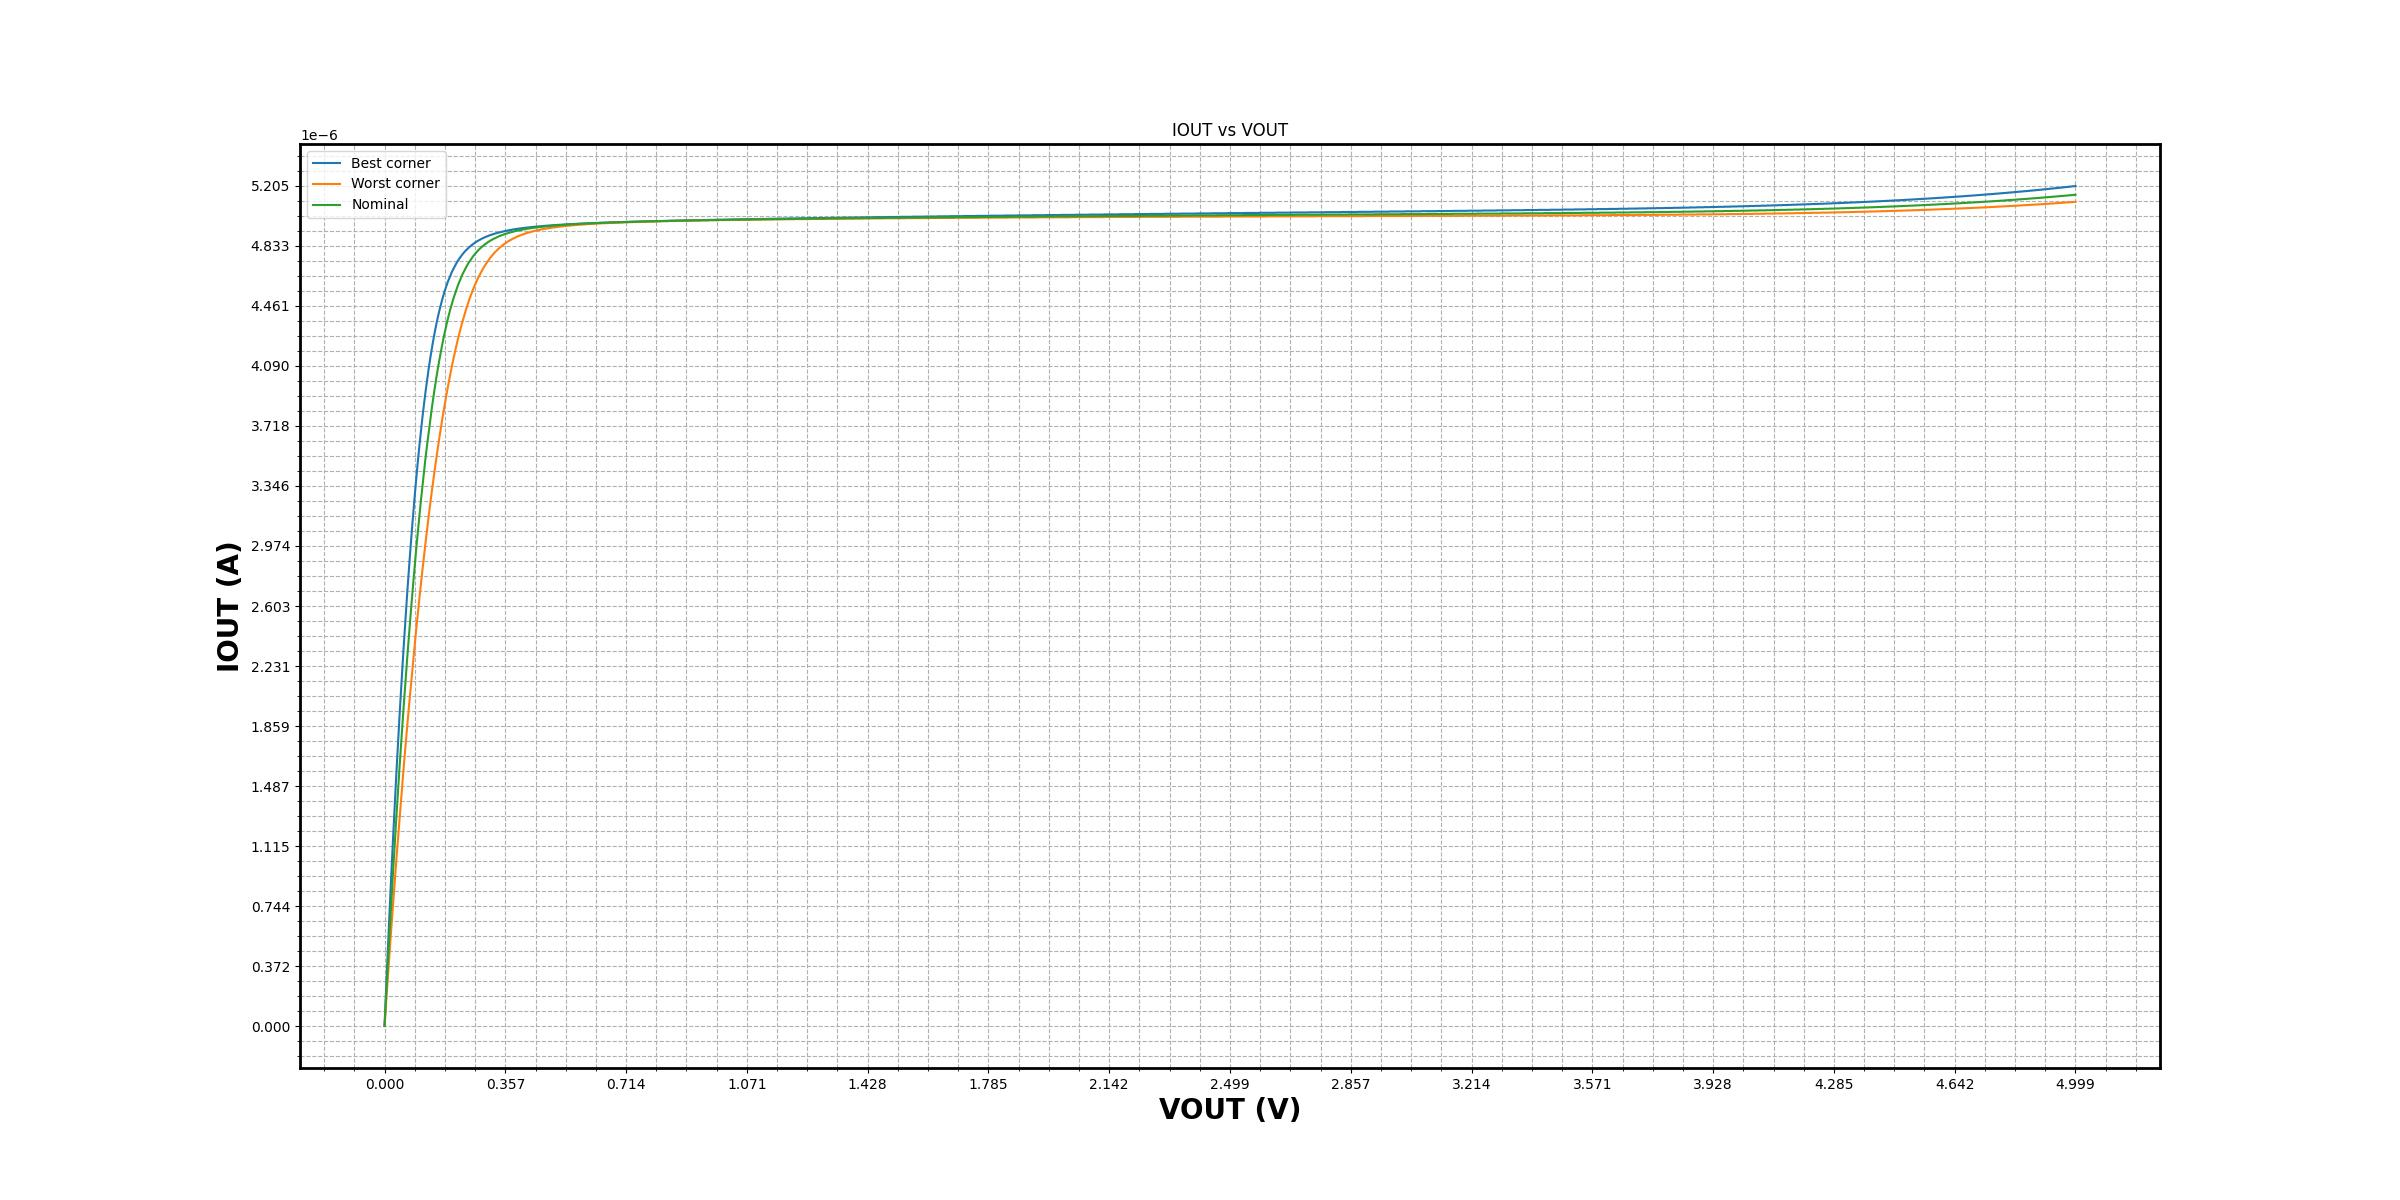
\includegraphics[width=.7\textwidth]{./IOUT_vs_VOUT.jpg} % Assuming this is the image generated by your Python script
    \caption{IOUT vs VOUT}
    \label{fig:iout_vs_vout}
\end{figure}




Fig.\ref{fig:output_impedance} represent the output impedance characteristic fo nominal, worst and best case scenario.

\begin{figure}[H] % Use H option for float placement
    \centering
    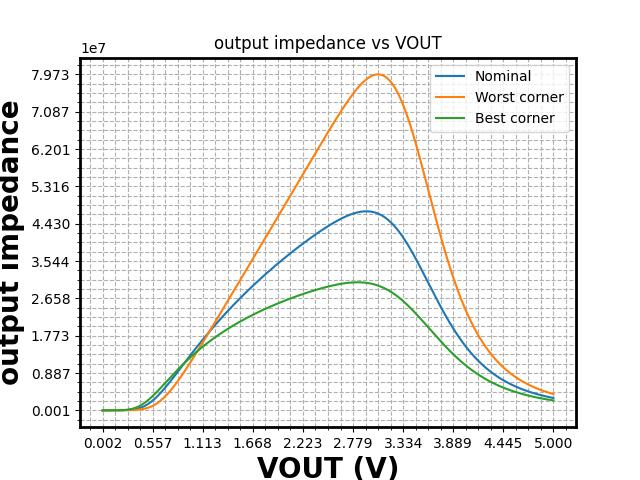
\includegraphics[width=.7\textwidth]{./output_impedance_vs_VOUT.jpg} % Assuming this is the image generated by your Python script
    \caption{output impedance}
    \label{fig:output_impedance}
\end{figure}



Fig.\ref{fig:ac_current_variatioion} represent the current variation face an ac signal fo nominal, worst and best case scenario.

\begin{figure}[H] % Use H option for float placement
    \centering
    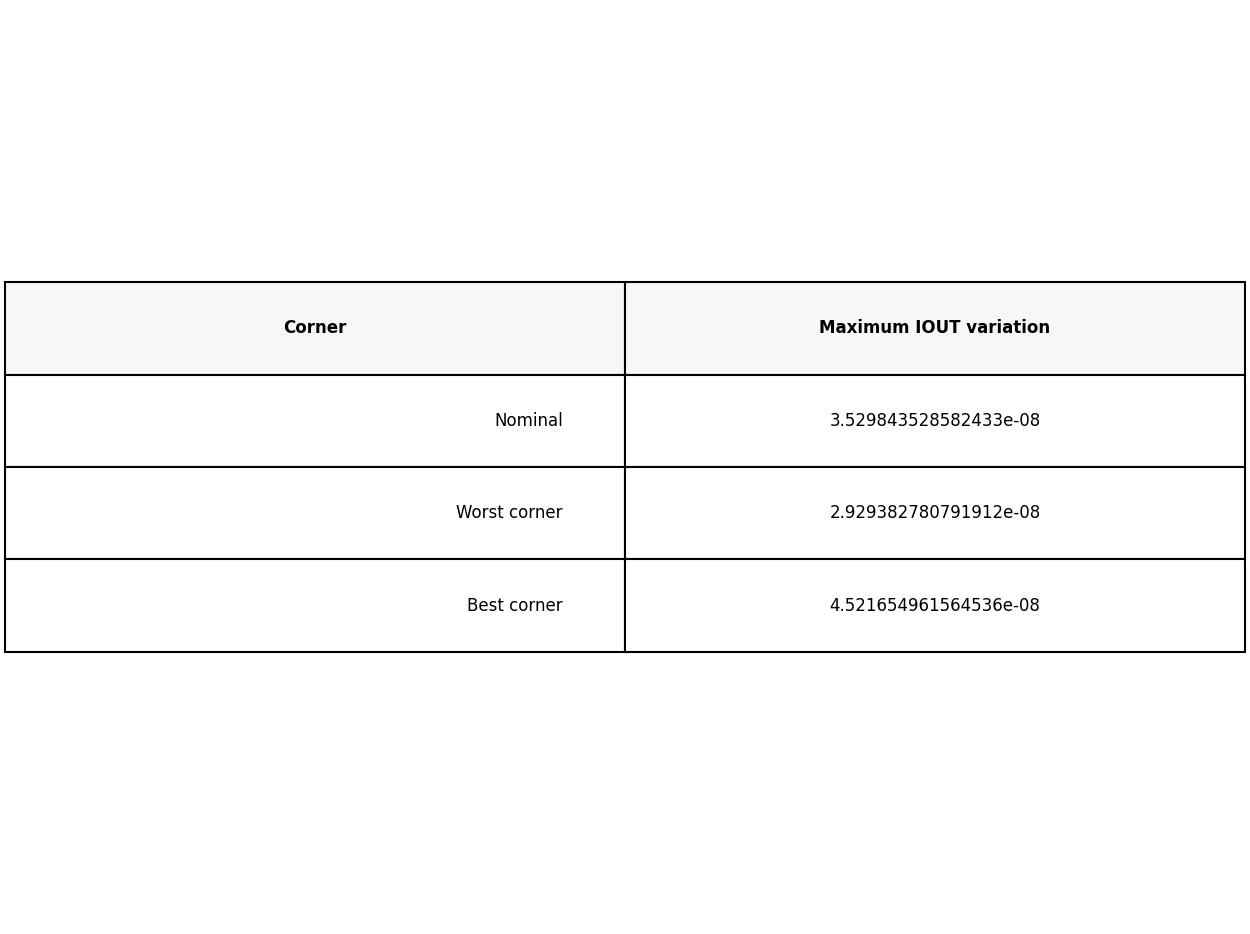
\includegraphics[width=.7\textwidth]{./ac_bias_table.jpg} % Assuming this is the image generated by your Python script
    \caption{ac variation}
    \label{fig:ac_current_variation}
\end{figure}

Fig.\ref{fig:nominal} represent the current variation at vout = VDD/2 with 200 runs.

\begin{figure}[H] % Use H option for float placement
    \centering
    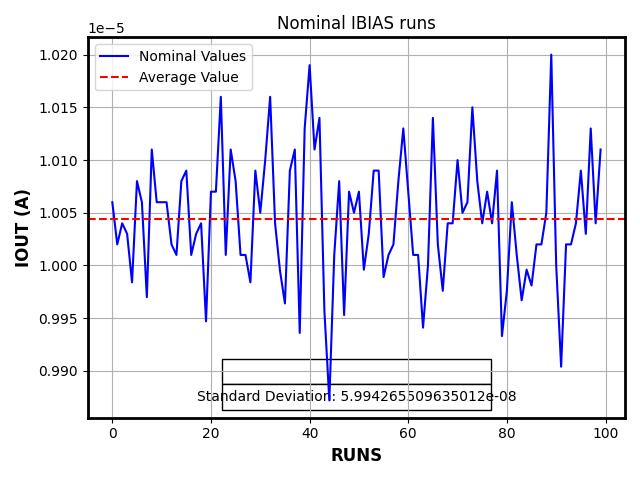
\includegraphics[width=.7\textwidth]{./Nominal_IBIAS_runs.jpg} % Assuming this is the image generated by your Python script
    \caption{Monte carclo variations}
    \label{fig:nominal}
\end{figure}


Fig.\ref{fig:histogram} represent the histogram.

\begin{figure}[H] % Use H option for float placement
    \centering
    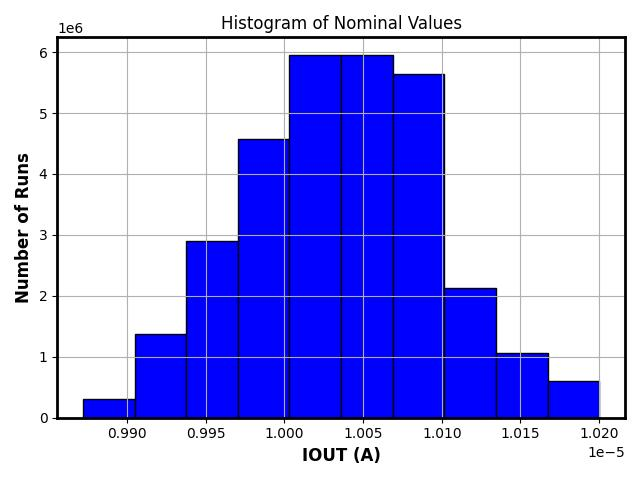
\includegraphics[width=.7\textwidth]{./Nominal_IBIAS_runs_histogram.jpg} % Assuming this is the image generated by your Python script
    \caption{Monte carclo variations}
    \label{fig:histogram}
\end{figure}


\section{load and VOUT characteristics}
Load impedance with the bias generator, determines the dc value of vout, to this cae we center its value to VDD/2 at 27 degrees at tt corner. Fig.\ref{fig:table_vout} shows the dispersion of VOUT at the worst corners.

\begin{figure}[H] % Use H option for float placement
    \centering
    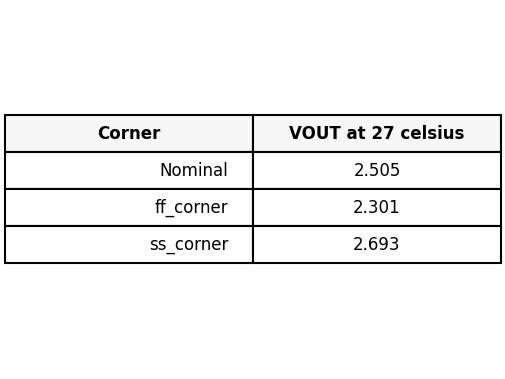
\includegraphics[width=.7\textwidth]{./only_PMOS_LOAD_VDC_NMOS_table.jpg} % Assuming this is the image generated by your Python script
    \caption{VOUT defenition in fucntion of the load}
    \label{fig:table_vout}
\end{figure}

Fig.\ref{fig:vout_temp_var}  shows the variation of VOUT in fucntion of temperature.

\begin{figure}[H] % Use H option for float placement
    \centering
    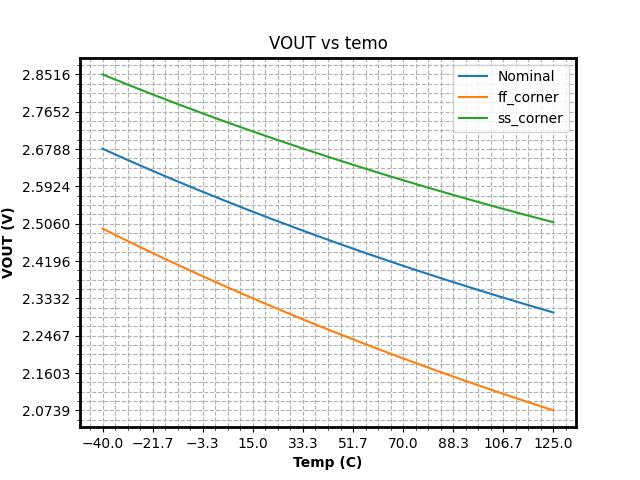
\includegraphics[width=.7\textwidth]{./only_PMOS_LOAD_VDC_NMOS.jpg} % Assuming this is the image generated by your Python script
    \caption{VOUT defenition in function of the temperature}
    \label{fig:vout_temp_var}
\end{figure}




Fig.\ref{fig:vout_temp_var}  shows the variation of VOUT in fucntion of a monte carlo simulation.

\begin{figure}[H] % Use H option for float placement
    \centering
    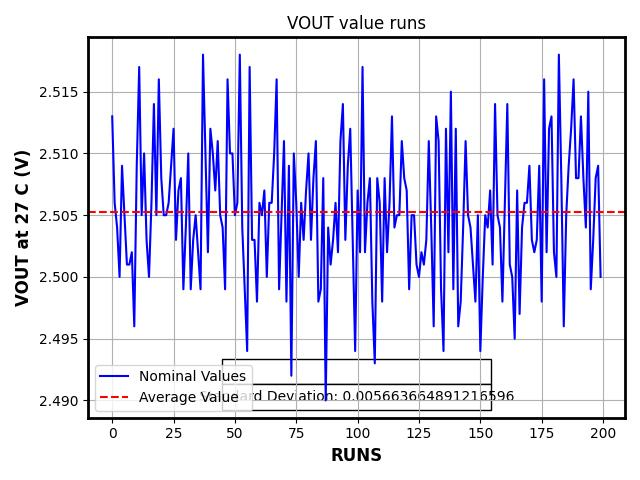
\includegraphics[width=.7\textwidth]{./VOUT_value_runs.jpg} % Assuming this is the image generated by your Python script
    \caption{VOUT vs monte carlo}
    \label{fig:vout_temp_var_hist}
\end{figure}




Fig.\ref{fig:vout_temp_var}  shows the variation of VOUT in fucntion of a monte carlo simulation in histogram form.

\begin{figure}[H] % Use H option for float placement
    \centering
    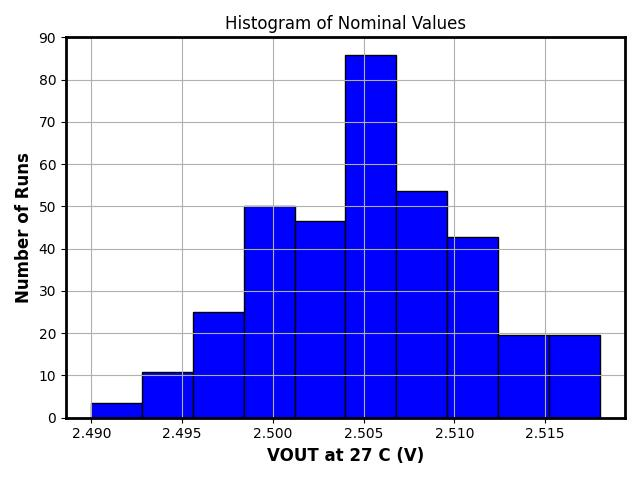
\includegraphics[width=.7\textwidth]{./VOUT_value_runs_histogram.jpg} % Assuming this is the image generated by your Python script
    \caption{VOUT vs monte carlo histogram}
    \label{fig:vout_temp_var_hist}
\end{figure}




\end{document}